%\title{Modelo de Projeto de pesquisa}
%% abtex2-modelo-projeto-pesquisa.tex, v-1.9 laurocesar
%% Copyright 2012-2013 by abnTeX2 group at http://abntex2.googlecode.com/ 
%%
%% This work may be distributed and/or modified under the
%% conditions of the LaTeX Project Public License, either version 1.3
%% of this license or (at your option) any later version.
%% The latest version of this license is in
%%   http://www.latex-project.org/lppl.txt
%% and version 1.3 or later is part of all distributions of LaTeX
%% version 2005/12/01 or later.
%%
%% This work has the LPPL maintenance status `maintained'.
%% 
%% The Current Maintainer of this work is the abnTeX2 team, led
%% by Lauro César Araujo. Further information are available on 
%% http://abntex2.googlecode.com/
%%
%% This work consists of the files abntex2-modelo-projeto-pesquisa.tex
%% and abntex2-modelo-references.bib
%%

% ------------------------------------------------------------------------
% ------------------------------------------------------------------------
% abnTeX2: Modelo de Projeto de pesquisa em conformidade com 
% ABNT NBR 15287:2011 Informação e documentação - Projeto de pesquisa -
% Apresentação 
% ------------------------------------------------------------------------ 
% ------------------------------------------------------------------------

\documentclass[
	% -- opções da classe memoir --
	12pt,				% tamanho da fonte
	openright,			% capítulos começam em pág ímpar (insere página vazia caso preciso)
	oneside,			% para impressão em verso e anverso. Oposto a oneside
	a4paper,			% tamanho do papel. 
	% -- opções da classe abntex2 --
	%chapter=TITLE,		% títulos de capítulos convertidos em letras maiúsculas
	%section=TITLE,		% títulos de seções convertidos em letras maiúsculas
	%subsection=TITLE,	% títulos de subseções convertidos em letras maiúsculas
	%subsubsection=TITLE,% títulos de subsubseções convertidos em letras maiúsculas
	% -- opções do pacote babel --
	english,			% idioma adicional para hifenização
	french,				% idioma adicional para hifenização
	spanish,			% idioma adicional para hifenização
	brazil,				% o último idioma é o principal do documento
	]{abntex2}

% ---
% PACOTES
% ---

% ---
% Pacotes fundamentais 
% ---
\usepackage{lmodern}			% Usa a fonte Latin Modern
\usepackage[T1]{fontenc}		% Selecao de codigos de fonte.
\usepackage[utf8]{inputenc}		% Codificacao do documento (conversão automática dos acentos)
\usepackage{indentfirst}		% Indenta o primeiro parágrafo de cada seção.
\usepackage{color}				% Controle das cores
\usepackage{graphicx}			% Inclusão de gráficos
\graphicspath{ {./} }
\usepackage{microtype} 			% para melhorias de justificação
\usepackage{multirow}			% para tabelas com celulas mergeadas
\usepackage{array}			% para multilinhas nas celulas

% ---

\newcolumntype{L}{>{\centering\arraybackslash}m{1cm}}

% ---
% Pacotes adicionais, usados apenas no âmbito do Modelo Canônico do abnteX2
% ---
\usepackage{lipsum}				% para geração de dummy text
% ---

% ---
% Pacotes de citações
% ---
\usepackage[brazilian,hyperpageref]{backref}	 % Paginas com as citações na bibl
\usepackage[alf]{abntex2cite}	% Citações padrão ABNT

% --- 
% CONFIGURAÇÕES DE PACOTES
% --- 

% ---
% Configurações do pacote backref
% Usado sem a opção hyperpageref de backref
\renewcommand{\backrefpagesname}{Citado na(s) página(s):~}
% Texto padrão antes do número das páginas
\renewcommand{\backref}{}
% Define os textos da citação
\renewcommand*{\backrefalt}[4]{
	\ifcase #1 %
		Nenhuma citação no texto.%
	\or
		Citado na página #2.%
	\else
		Citado #1 vezes nas páginas #2.%
	\fi}%
% ---

% ---
% Informações de dados para CAPA e FOLHA DE ROSTO
% ---
\titulo{Coletando dados de memória de uma máquina em nuvem para análise forense}
\autor{Hamilton Fonte II}
\orientador{Marcos Antonio Simplício Jr}
\local{São Paulo, Brasil}
\data{2016, v-0.1}
\instituicao{%
  Universidade de São Paulo -- USP
  \par
  Escola Politécnica - Engenharia de Computação
  \par
  Programa de Pós Graduação em Engenharia Elétrica - Mestrado}
\tipotrabalho{Plano de Pesquisa de Pós-Graduação - Mestrado}
% O preambulo deve conter o tipo do trabalho, o objetivo, 
% o nome da instituição e a área de concentração 
\preambulo{Projeto de pesquisa para a disciplina Metodolodia de Pesquisa 
Científica em Engenharia de Computação.}
% ---

% ---
% Configurações de aparência do PDF final

% alterando o aspecto da cor azul
\definecolor{blue}{RGB}{41,5,195}

% informações do PDF
\makeatletter
\hypersetup{
     	%pagebackref=true,
		pdftitle={\@title}, 
		pdfauthor={\@author},
    	pdfsubject={\imprimirpreambulo},
	    pdfcreator={LaTeX with abnTeX2},
		pdfkeywords={abnt}{latex}{abntex}{abntex2}{projeto de pesquisa}, 
		colorlinks=true,       		% false: boxed links; true: colored links
    	linkcolor=blue,          	% color of internal links
    	citecolor=blue,        		% color of links to bibliography
    	filecolor=magenta,      		% color of file links
		urlcolor=blue,
		bookmarksdepth=4
}
\makeatother
% --- 

% --- 
% Espaçamentos entre linhas e parágrafos 
% --- 

% O tamanho do parágrafo é dado por:
\setlength{\parindent}{1.3cm}

% Controle do espaçamento entre um parágrafo e outro:
\setlength{\parskip}{0.2cm}  % tente também \onelineskip

% ---
% compila o indice
% ---
\makeindex
% ---

% ----
% Início do documento
% ----
\begin{document}

% Retira espaço extra obsoleto entre as frases.
\frenchspacing 

% ----------------------------------------------------------
% ELEMENTOS PRÉ-TEXTUAIS
% ----------------------------------------------------------
% \pretextual

% ---
% Capa
% ---
\imprimircapa
% ---

% ---
% Folha de rosto
% ---
\imprimirfolhaderosto
% ---

% ---
% NOTA DA ABNT NBR 15287:2011, p. 4:
%  ``Se exigido pela entidade, apresentar os dados curriculares do autor em
%     folha ou página distinta após a folha de rosto.''
% ---

% ---
% inserir o sumario
% ---
\tableofcontents
\cleardoublepage
% ---


% ----------------------------------------------------------
% ELEMENTOS TEXTUAIS
% ----------------------------------------------------------
\textual

% ----------------------------------------------------------
% Introdução
% ----------------------------------------------------------
\chapter{Introdução}

Aqui vai a introdução

% ----------------------------------------------------------
% Capitulo de justificativa 
% ----------------------------------------------------------
\chapter{Justificativa}

Aqui vai a justificativa

% ----------------------------------------------------------
% Capitulo de Objetivos 
% ----------------------------------------------------------
\chapter{Objetivos}

Aqui vão os objetivos

% ----------------------------------------------------------
% Capitulo de Minha solução 
% ----------------------------------------------------------
\chapter{Minha Solução}

\textbf{Motivações}

Aumento do uso de soluções de virtualização e a implementação de arquiteturas em nuvem que escalam automáticamente \cite{Amazon2016} trouxe a questão da volatilidade 
das máquinas virtuais. Uma aplicação hospedada na nuvem sob um pico de uso pode clonar máquinas e adiciona-las ao grupo para atender a demanda. Passado 
este pico, as máquinas que foram clonadas são despejadas, seus recursos liberados e o conjunto de retorna ao tamanho inicial. Com as ameaças que atuam diretamente 
na memória sem deixar rastros no disco da máquina afetada, se essas máquinas forem usadas para algum evento ilícito, as evidências do acontecimento contidas nelas 
serão para sempre perdidas.

Para o escopo deste trabalho estamos considerando 4 tipos de ataques realizados diretamente na memória e que não deixam rastros no disco da máquina, todos baseados 
em injeção de código \cite{Case2014}.

\begin{itemize}
 \item \textbf{Injeção remota de bibliotecas} - Um processo malicioso força o processo alvo a carregar uma biblioteca em seu espaço de memória através de comandos do sistema operacional.
 A biblioteca existe fisicamente em alguma localização remota.
 \item \textbf{Injeção remota de código} - Um processo malicioso escreve código como uma sequência de bytes diretamente no espaço de memória de um processo alvo e força este 
 último a executa-lo. O código pode por exemplo ser um script de shell
 \item \textbf{Injeção reflexiva de biblioteca} - Um processo malicioso escreve diretamente na memória de um processo alvo, como uma sequência de bytes, o código de uma biblioteca
 e força o processo alvo a executa-la. Nesta forma de ataque a biblioteca não existe fisicamente.
 \item \textbf{Injeção de processo vazio} - Um processo malicioso dispara uma instância de um processo legítimo no estado suspenso, a área do executável é liberada e realocada com 
 código malicioso.
\end{itemize}

Do ponto de vista forense, praticantes e pesquisadores concordam aspectos de multi-inquilino e multi-jurisdição próprios soluções em nuvem figuram entre as principais 
dificuldades para coleta de evidência \cite{Bash2015a}. O aspecto multi-inquilino impede a remoção do hardware pois como ele é compartilhado com vários usuários, 
removê-los seria uma violação de privacidade de usuários não relacionados a investigação. Por fim a característica distribuída pode alocar informação relevante a 
investigação em vários países dificultando a obtenção da mesma \cite{Dykstra2012a}.

O crescente volume de dados das aplicações atuais deram aos investigadores em média de 6 a 12 meses de backlog para investigar \cite{Quick2014}, download de terabytes
de dados leva horas para se realizar e requer a colaboração do provedor de nuvem. Mudar o paradigma de coleta tem sido proposto por pesquisadores e praticantes já há alguns
anos \cite{Birk2011}\cite{Sang2013} mas estas práticas precisam garantir a cadeia de custódia para que as evidências produzidas por ela sejam aceita em um processo legal.\\

\textbf{Objetivos da solução}

\begin{itemize}
 \item Coletar memória de uma máquina virtual de modo a conseguir identificar os 4 tipos de ataque listados anteriormente.
 \item Coletar memória de uma máquina virtual de modo a conseguir identificar sua fonte mesmo se a máquina virtual não existir mais.
 \item Coletar memória suficiente para conseguir descrever o sistema antes e depois do incidente.
 \item Armazenar a memória coletada de modo a garantir sua integridade, confidencialidade, não violar jurisdição e não violar privacidade de outros usuários no host.\\
\end{itemize}

\textbf{Descrição da solução}

Nas soluções com infra-estrutura física a máquina é persistente. Associar uma copia da memória, a imagem de um disco ou pacotes trafegando na rede a uma máquina é tarefa simples.
Com as soluções de infra virtual, em especial as auto-escaláveis, a máquina deixou de ser persistente e tornou-se volátil. Para resolver o problema da identificação da fonte
precisamos encontrar outra forma persistente para identificar a fonte da evidência coletada. Para isto usamos containeres. Embora o container seja uma peça de software e 
por consequência também é volátil, a imagem compilada e sua execução na forma de container estão atrelados a um hash que os identificam, a pilha de um container pode ser 
visto na Figura 1. 

\begin{figure}[h]
\caption{Pilha monstrando funcionamento de container}
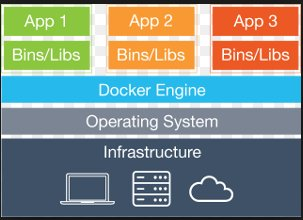
\includegraphics[scale=0.5]{docker.jpg}
\centering
\label{fig:instantaneo}
\end{figure}

A solução proposta por este trabalho, para resolver o problema de associação da evidência a sua origem de modo que o processo seja reprodutível, pausa a execução
do container e coleta um instantâneo da memória dos processos sob sua execução. Este processo é executado em intervalos de tempo conhecidos de modo a se ter uma
evolução da história da memória dos processos. Em um sistema derivado do linux (Ubuntu 14.04) isso foi atingido via cópia do diretório ``\\proc'' relacionado 
aos processos sob o ``cgroup'' associado ao container e salvo em disco. Para relacionar o instantâneo a sua origem, usamos como nome do arquivo contendo o instantâneo 
da memória a combinação do hash da imagem e o hash do container como mostrado na Figura 2.

\begin{figure}[h!]
\caption{Evidência salva - hash do container e imagem}
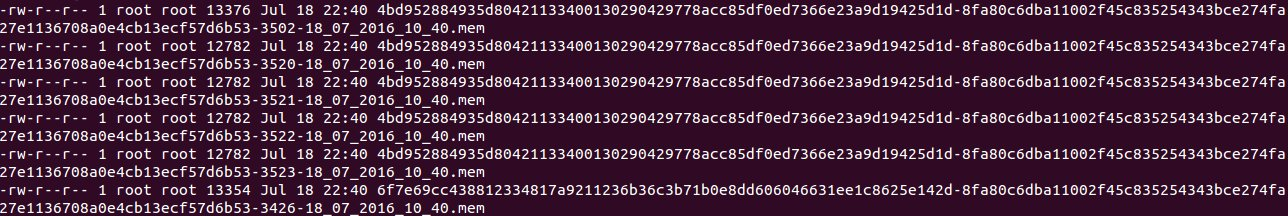
\includegraphics[scale=0.3]{snapshot.jpg}
\centering
\label{fig:instantaneo}
\end{figure}

As técnicas forenses praticadas hoje estão voltadas para a obtenção da informação em sua totalidade, seja via cópia bit a bit, seja por remoção do hardware \cite{Simou2014}
\cite{Bem2008}. Tais práticas tem levado ao crescente volume de dados que os investigadores tem que analisar. Há uma vertente na comunidade chamada ``sniper 
forensics'' onde se coleta e armazena o suficiente para a investigação. A solução proposta por este trabalho acompanha esta tendência, a questão foi definir a quantidade 
de dados ``suficiente'' para uma investigação. Decidimos que ``suficiente'' seria a quantidade necessária para descrever o sistema antes e depois do ataque. A idéia é 
implementar um log rotativo de instantâneos de memória cobrindo uma quantidade de tempo configurável, integrar a solução com algum sistema de detecção de ameaça de modo
que, ao detectar um ataque, o log passa de rotativo a completo assim permitindo que se conheça o sistema antes e depois do ataque como mostrado na Figura 3. 

\begin{figure}[h!]
\caption{Janela deslizante de coleta de evidência}
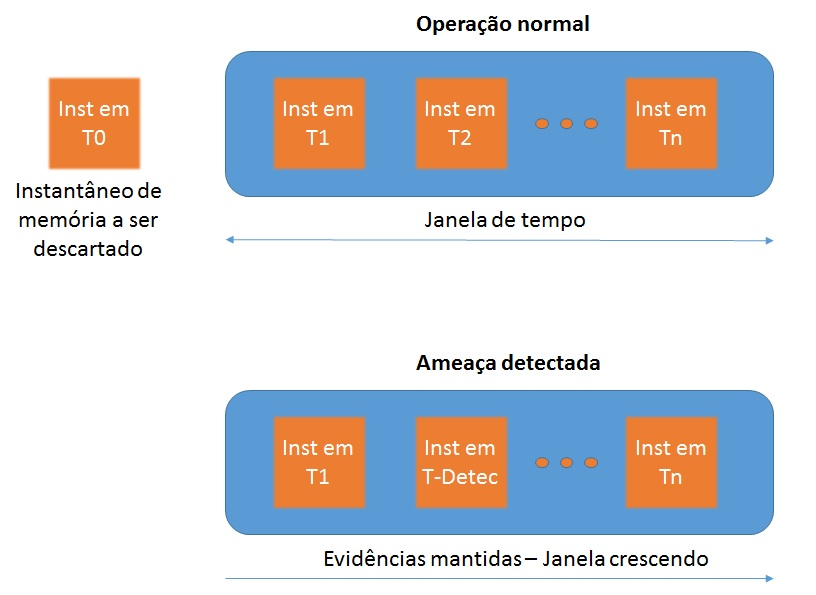
\includegraphics[scale=0.5]{janela.jpg}
\centering
\label{fig:janela}
\end{figure}

De modo a não violar a jurisdição de outros países ou a privacidade de outros usuários por causa do caráter multi-inquilino e multi-jurisdição das arquiteturas em núvem pública,
a solução proposta por este trabalho foi o de armazenar a evidência em um local físico fora da nuvem utilizando como transporte conexão segura. Outro ponto importante é 
garantir a cadeia de custódia da evidência ou seja, garantir que a evidência não foi destruída, alterada ou acessada por qualquer pessoa. Assim a solução proposta por este 
trabalho usará de armazenamento físico fora da nuvem, o transporte será feito por TLS e o acesso a evidência será controlado.

Tendo a implementação sido bem sucedida conseguiremos analisar e identificar as formas de ataque enumeradas nos objetivos.\\

\textbf{Limitações da solução}

Ameaças das quais estamos focando neste trabalho usam técnicas que permitem passar desapercebidas pelo processo de detecção de ameaças. Algumas delas são, 
adulteração da lista de processos ativos em uma máquina, se fazer passar por um processo válido ou se fazer passar por uma biblioteca válida \cite{Case2014}. Por isso, 
mesmo que haja uma integração com alguma forma de detecção de ameaça para a mudança do armazenamento de janela para o armazenamento total, acreditamos que ainda é 
necessária a capacidade de acionamento manual.

A solução esta focada em coletar informações de memória do espaço de memória do usuário assim, mesmo que ela ajude na investigação de ameaças que realizem manipulação direta
dos objetos do Kernel ( \textit{D.K.O.M. - Direct Kernel Object Manipulation} ) Kernel space no host não se beneficia da associação com o container.\\

\textbf{Esquema da solução}

A solução completa com todos os elementos descritos anteriormente pode ser visto na figura 4

\begin{figure}[h]
\caption{Solução completa}
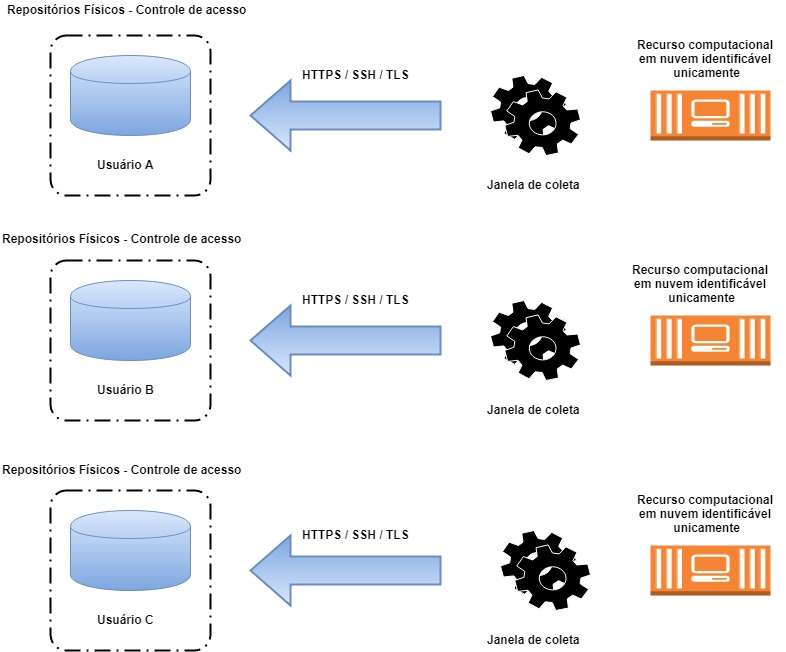
\includegraphics[scale=0.5]{solucao.jpg}
\centering
\label{fig:Solucao}
\end{figure}

% ----------------------------------------------------------
% Plano de Trabalho 
% ----------------------------------------------------------
\chapter{Métodos}

Aqui vão os métodos

% ----------------------------------------------------------
% Material e métodos
% ----------------------------------------------------------
\chapter{Revisão Bibliográfica}

\begin{itemize}

\item \textbf{Digital forensics framework for a cloud environment \cite{George2012} }: Arcabouço para coleta de dados de máquinas virtuais. Possui duas formas de 
acionamento, a manual e a automática, integrada com algum sistema de detecção de ameaça. Quando acionado, escuta a rede, determina qual máquina é objeto de investigação, 
coleta informações de log e tráfego de rede e associa ao usuário da respectiva máquina. Propõe o armazenamento das evidências em local fora da núvem para escapar de 
problemas de jurisdição e multi-inquilino mas tem inteligência para usar a própria nuvem como armazenamento caso o espaço fora acabe.

A proposta dá a entender que é aplicável apenas a um sistema virtual estático, onde o número e organização das máquinas é constante. De informação volátil coleta apenas 
tráfego de rede, não coleta memória. Com a forma de acionamento descrito ele não consegue descrever, com as evidências, como era o sistema antes do ataque. Apesar de armazenar 
a evidência fora da nuvem, não da detalhes de como garante que a evidência não foi alterada ou destruída no transporte até o local de armazenamento nem como controla o 
acesso a evidência.

Quando comparado a este trabalho, a presente proposta tem por vantagens a utilização de container para associar a evidência a sua origem tornando o processo independente 
de máquina e permitindo que seja repetido mesmo se a máquina de onde se originaram os dados não existir mais. Com a implementação de uma janela de x dias de coleta antes da
detecção do ataque é possível descrever, através de evidência, como era o sistema antes do mesmo. Com isso a solução apresentada consegue evidências em um cenário de
infra-estrutura dinâmica. São tomadas precauções para garantir que os dados não foram alterados ou destruídos no transporte via TLS os para um local fora da nuvem e 
o acesso a mesma é controlado.\\
 
\item \textbf{Evidence and cloud computing the virtual machine introspection approach \cite{Poisel2013} }: Descreve um método de coleta de informações de máquinas
em nuvem através da técnica de introspecção em máquina virtual, onde se acessa os dados das máquinas virtuais através do hypervisor. Propõe que o processo seja disparado
automaticamente integrado a um sistema de detecção de ameaça mas também suporta acionamento manual.

A técnica descrita cobre apenas o processo de coleta de informações, não explica onde ou como elas serão armazenadas. No que tange as informações de memória, como os 
endereços de memória são os do host, estes precisam ser traduzidos para que a análise forense seja feita. Segundo a comunidade, tal estratégia é imune a técnicas anti-
forenses empregadas por usuários maliciosos pois está localizada fora da máquina virtual. Como a abordagem não tem conhecimento do que está rodando dentro da máquina 
precisa de uma copia bit a bit da evidência. Embora pareça possível, não descreve como lida com o cenário onde uma máquina é despejada do pool e os recursos liberados. 

Quando comparado a este trabalho, a presente proposta tem por vantagens ser um arcabouço para coleta e armazenamento de evidências. Usa-se uma estratégia 
diferente pois coleta-se a memória diretamente de dentro da máquina virtual onde se evita o problema do gap semântico próprio das soluções por introspecção. 
Como não precisa realizar tradução de endereços, a presente proposta consegue realizar uma coleta onde os dados já são úteis para análise e pode direcionar a mesma
pois tem o conhecimento do que está rodando na máquina. De acordo com a comunidade é mais sucetível a técnicas anti-forenses.\\

\item \textbf{Design and implementation of FROST: FoRensic tools for Open STack \cite{Dykstra2013} }: Arcabouço para coleta de dados de máquinas virtuais através da API do
hypervisor. Isola a máquina virtual afetada do pool original para realização da coleta. Precisa ser acionado quando uma ameaça é detectada. É o mais bem acabado arcabouço de
todas as propostas encontradas até agora mas ao detalhar o processo de armazenamento não explica como garante que a evidência não será destruida ou alterada no transporte
até o armazenamento nem como controla o acesso a evidência. Por estar integrado ao Open Stack o arcabouço depende de cooperação do provedor de serviços de nuvem onde ele 
está rodando, isso é considerado problemático pela comunidade pois a prioridade do mesmo é manter o serviço funcionando e não coletar evidencias forenses. Como está na
mesma camada do hypervisor não conhece o que está rodando dentro da máquina. Depende da existência da máquina virtual para realização da coleta.

Quando comparado a este trabalho, a presente proposta tem por vantagens a utilização de container para associar a evidência a sua origem tornando o processo 
independente de máquina e permitindo que seja repetido mesmo se a máquina de onde originaram os dados não existir mais. Coma implementação de uma janela 
de x dias de coleta antes da detecção do ataque é possível descrever, através da evidência, como era o sistema antes do mesmo. Não depende de cooperação do provedor 
do serviço de nuvem. A presente proposta também consegue realizar uma coleta onde os dados já são úteis para análise e pode direcionar a mesma pois tem o conhecimento 
do que está rodando na máquina. \\
  
\item \textbf{Automated Forensic Data Acquisition in the Cloud \cite{Reichert2015} }: Propõe um modelo que tira instantâneos de máquinas virtuais atrelado a algum mecanismo de
detecção de ameaça baseado no hypervisor. Usa o Google Rapid Response para salvar as informações coletadas fora da núvem de forma a driblar os problemas de multi-jurisdição e 
multi-inquilino. Descreve satisfatóriamente como evita que a evidência seja alterada ou destruída no transporte até o armazenamento e como controla o acesso a evidência.

O modelo proposto só começa a coletar evidência após a detecção da ameaça e toma um instantâneo da máquina toda o que já foi julgado pela comunidade como um processo custoso em
termos de espaco em disco e piora o problema do volume de dados a ser analisado. Pessoalmente acho arriscado depender de instantâneos pois caso precise, repetir o processo de coleta
pode não ser possível. Um exemplo é editar um disco virtual que estava atrelado a uma máquina virtual da qual se gerou os instantâneos, tal ação pode levar a perda de dados.

Como métrica, o autor relaciona o tamanho da memória alocada na máquina virtual com o tempo necessário para gerar o instantâneo de acordo com a tabela 1 abaixo

\begin{table}[h!]
\centering
\caption{Memória alocada X Tempo de captação}
\label{my-label}
\begin{tabular}{c|c}
\hline
\textbf{Memória alocada na VM} & \textbf{Tempo geração snapshot} \\ \hline
512 Mb                         & 15 segundos                     \\ \hline
1 Gb                           & 20 segundos                     \\ \hline
4 Gb                           & 36 segundos                     \\ \hline
\end{tabular}
\end{table}

Quando comparado a este trabalho, a presente proposta tem por vantagens coletar apenas a informações de memória e usar a janela de coleta de \textbf{x} dias antes do ataque para 
manter sob controle a quantidade de informação que precisa ser analisada. Tomando como referência a tabela acima, conseguiremos um menor tempo de coleta da informação de 
memória pertinente a investigação, permitindo um menor espaço de tempo entre as coletas, gerando menos impacto na performance da aplicação e mais dados para a investigação.
Propondo a autilização de container para associar a evidência a sua origem, tornamos o processo independente de máquina. \\
 
\item \textbf{A log based approach to make digital forensics easier on cloud computing \cite{Sang2013} }: Método sugere salvar a informação coletada fora da núvem de modo 
a driblar os problemas de multi-inquilinato e multi-jurisdição, usa um mecanismo de hash para garantir a autenticidade e integridade da informação mas não dá detalhes da 
implementação e não descreve como controla o acesso a evidência armazenada. Segundo o próprio autor, o método não funciona em IaaS. Precisa da cooperação do provedor de 
nuvem pois depende das informações que este último decidiu adicionar ao log. O método não é aplicável a coleta de informações de memória.

A proposta não coleta dados de memória por decisão do autor, esta proposta entrou na lista pela abordagem baseada em log. Neste quesito, a presente proposta é a melhor pois 
garante que a evidência não foi alterada ou destruida no transporte e o acesso a mesma é controlado. No âmbito da informação coletada, a presente proposta não depende das 
decisões do provedor de nuvem sobre o que guardar no log para conseguir a evidência. \\

\item \textbf{Volatile memory acquisition using backup for forensic investigation \cite{Dezfouli2012} }: Técnica desenvolvida para dispositivos móveis que sugere a utilização
do próprio como repositório das evidências coletadas da memória. Para manter a utilização de espaço ao mínimo sugere manter apenas o último estado conhecido da memória.
 
É uma técnica interessante do ponto de vista de estratégia de armazenamento quando guarda apenas o último estado da memória. Essa abordagem porém perde a informação do momento 
do ataque e não consegue descrever o sistema antes do mesmo. Do resto da proposta não é aplicável para este projeto pois, armazenando a evidência na máquina a mesma seria perdida
quando a máquina fosse despejada do pool e seus recursos liberados. A cadeia de custódia não é abordada na proposta.\\

\item \textbf{Narrowing the semantic gap in virtual machine introspection \cite{Dolan-Gavitt2011a} }: Esta proposta é uma combinação da técnica de introspecção em máquina virtual
e a integração com a API do hypervisor. O principal objetivo é diminuir o gap semântico para facilitar a análise da evidência. Para isso o autor implementa um API para transformar
dados de baixo nível em informação de alto nível. Depende de cooperação do provedor de serviço de nuvem, não tem conhecimento da máquina hospedada e não vai além da coleta, não 
descreve como resolve a cadeia de custódia. Tem a vantagem de ser imune a técnicas anti-forenses.

Como métrica o autor relaciona o tamanho médio do trace gerado a partir da uma evidência de memória coletada de alguns processos em vários sistemas operacionais de acordo 
com a tabela 2 abaixo. Essa métrica pode se relacionar a presente proposta como o volume de informação extraida de uma evidência.

\begin{table}[]
\centering
\caption{Tamanho do trace coletado de vários programas}
\label{my-label}
\begin{tabular}{l|c|c}
\hline
\textbf{Sistema Operacional}		&\textbf{Programa}	      & \textbf{Tamanho do Trace}\\ \hline
\multirow{6}{*}{Windows}                & getpid                      & 3549			 \\
                                        & gettime                     & 7715    		 \\
                                        & pslist                      & 302082  		 \\
                                        & lsmod                       & 195488   		 \\
                                        & getpsfile                   & 49588   		 \\
                                        & getdrvfile                  & 194765  		 \\
\multirow{5}{*}{Linux}                  & getpid                      & 133047                   \\ \hline
                                        & gettime                     & 75074                    \\
                                        & pslist                      & 6107214                  \\
                                        & lsmod                       & 1936439                  \\
                                        & getpsfile                   & 14752561                 \\
\multirow{6}{*}{Haiku}                  & getpid                      & 18242                    \\ \hline
                                        & gettime                     & 9982                     \\
                                        & pslist                      & 362127                   \\
                                        & lsmod                       & 850363                   \\
                                        & getpsfile                   & 249663                   \\
                                        & getdrvfile                  & 522299                   \\ 
\end{tabular}
\end{table}

Quando comparado a este trabalho, a presente proposta tem por vantagens ser arcabouço de coleta e armazenamento de evidências não apenas um método de coleta. Empregando a
estratégia de realizar a coleta diretamente na máquina não tem o problema do gap semântico próprio das soluções baseadas em introspecção. Como conhece o contexto do que 
está rodando dentro da máquina virtual podemos direcionar a coleta de modo que seja mais eficiênte. O autor usa outras métricas voltadas ao processamento da evidência antes
de sua análise para diminuir a quantidade de informação a se analisar mas não dá detalhes de como esse processamento.\\

\item \textbf{Digital Forensics as a Service: A game changer \cite{VanBaar2014} }: Esta proposta é focada em uma mudança no armazenamento e forma de trabalho dos peritos forenses.
Propõe que a forense seja oferecida como um serviço e que as evidências sejam armazenadas em um local centralizado com o devido controle de acesso e garantia de integridade da 
evidência. Descreve a arquitetura de armazenamento, qual o perfil que deve ter acesso a evidência e como é este acesso. Esta proposta não é focada apenas em incidentes na nuvem
mas em qualquer outro incidente.

Embora seja uma ótima proposta de armazenamento de evidências e controle de acesso a elas, ele não descreve o processo de coleta nem de transporte. É uma proposta focada 
mais na solução de problemas relacionados a manipulação da informação após a coleta, transporte e armazenamento. Não toca no assunto de coleta qualquer que seja, em nuvem
ou fisica.\\

\item \textbf{Live Digital Forensics in a Virtual Machine \cite{Zhang2010} }: Proposta para coletar informações de memória de máquinas virtuais através de instantâneos das mesmas.
O metodo de coleta envolve tomar o instantâneo da máquina, no diretório onde o mesmo foi armazenado pegar o arquivo referente a memória e abri-lo / analisá-lo usando um programa de
leitura de memória de mercado. O autor não trás detalhes do transporte, armazenamento ou controle de acesso. Precisa que a máquina exista para conseguir coletar a informação e 
o processo é dependente de intervenção humana. Analisando com mais cuidado é possível repetir a coleta mesmo sem a máquina existir uma vez que temos o instantâneo mas o autor não
dá detalhes do caso.

Quando comparado a este trabalho, a presente proposta tem por vantagens a menor quantidade de informação necessária à investigação através da implementação da janela de x
dias antes do incidente. Como o processo é automático, uma vez disparado não requer intervenção humana. A presente proposta descreve como garante a cadeia de custódia da 
evidência e consigue reproduzir o processo de coleta mesmo se a máquina não existir  mais pois a evidência está atrelada ao container.

\item \textbf{Comparative Analisys of volatile memory forensics \cite{Aljaedi2011} }: Levantamento sobre o impacto da realização de forense de memória ao vivo nas máquinas
virtuais na nuvem. Mostra que a quantidade de informações referentes a processos não alocados e página de memória perdida é um ponto a considerar quando se inicia uma
ferramente para análise de memória em uma máquina já funcionando como.

Como métrica o autor relaciona a porcentagem média de processos que permanecem na memória antes e depois que a ferramenta de coleta foi disparada com a quantidade de memória
alocada na VM de acordo com a tabela 3 abaixo.

\begin{table}[h!]
\centering
\caption{Média de processos que permaneceram na memória}
\label{my-label}
\begin{tabular}{c|c|c}
\hline
\textbf{Memória alocada a VM} & \textbf{\% antes da ativação} 			  & \textbf{\% depois da ativação} \\ \hline
1 Gb                          & 78,33                                             & 61,66                          \\ \hline
512 Mb                        & 73,33                                             & 46,66                          \\ \hline
256 Mb                        & 50,55                                             & 35,00                                                          
\end{tabular}
\end{table}

Em outra métrica o autor relaciona a porcentagem média de páginas de memória alterada nos métodos de \textbf{\% análise ao vivo}, onde a coleta é realizada com o sistema rodando e 
\textbf{\% cópia de memória} onde a máquina virtual é pausada para a realização de coleta de informação com a quantidade de memória alocada de acordo com a tabela abaixo. Em ambos
os casos as duas métricas são comparações entre o estado da memória antes e depois da inicialização da ferramenta de coleta.

\begin{table}[h!]
\centering
\caption{Média de página de memória alterada}
\label{my-label}
\begin{tabular}{c|c|c}
\hline
\textbf{Memória alocada a VM} & \textbf{\% análise ao vivo} 			  & \textbf{\% cópia de memória} \\ \hline
1 Gb                          & 7,99                                              & 5,95                         \\ \hline
512 Mb                        & 32,53                                             & 8,75                         \\ \hline
256 Mb                        & 52,37                                             & 25,46                                                         
\end{tabular}
\end{table}

Quando comparado a este trabalho a presente proposta tem por vantagem estar sempre em execução, sujeitando-se aos efeitos de escalonamento do processo e 
gerenciamento de páginas de memória pelo sistema operacional, assim não gera as perdas de informação de processos não alocados e páginas de memória referentes ao 
rearranjo que o kernel faz quando uma nova aplicação é iniciada.

\end{itemize}
 
\textbf{Tabela comparativa das soluções}
 
\begin{itemize}
 \item Digital forensic framework for a cloud environment - \textbf{A}
 \item Evidence and cloud computing. The virtual machine introspection approach - \textbf{B}
 \item Design and implementation of FROST: Digital forensic tools for Open Stack cloud computing platform - \textbf{C}
 \item Desafios da perícia forense em um ambiente de computação em núvem - \textbf{D}
 \item Automated data forensic acquisition in the cloud - \textbf{E}
 \item A log based approach to make digital forensics easier on cloud computing - \textbf{F}
 \item Narrowing the semantic gap in virtual machine introspection - \textbf{G}
 \item Comparative analisys of volatile memory forensics - \textbf{H}
 \item Volatile memory acquisition using backup for forensic investigation - \textbf{I}
 \item Digital forensics as a service, a game changer - \textbf{J}
\end{itemize}

 
\begin{table}[h!]
\centering
\caption{Comparativo de soluções}
\label{my-label}
\begin{tabular}{L|L|L|L|L|L|L}
\hline
\textbf{}	& \rotatebox{90}{\textbf{Coleta  é continua?}}      & \rotatebox{90}{\textbf{Precisa de tradução de endereços para análise?}}      & \rotatebox{90}{\textbf{É independente de VM?}}      & \rotatebox{90}{\textbf{Conhece o que esta rodando na VM?}}      & \rotatebox{90}{\textbf{Garante cadeia de custódia?}}      & \rotatebox{90}{\textbf{Preserva evidência de memória volátil?}}      \\ \hline
\textbf{A}	& Não                                               & Não                                                                          & Não                                                 & Sim                                                             & Não                                                       & Não                                                                  \\ \hline
\textbf{B}	& Não                                               & Sim                                                                          & Não                                                 & Não                                                             & Não                                                       & Sim                                                                  \\ \hline
\textbf{C}	& Não                                               & Não                                                                          & Não                                                 & Não                                                             & Não                                                       & Não                                                                  \\ \hline
\textbf{D}	& Não                                               & Não                                                                          & Não                                                 & Não                                                             & Não                                                       & Não                                                                  \\ \hline
\textbf{E}	& Não                                               & Não                                                                          & Não                                                 & Sim                                                             & Sim                                                       & Não                                                                  \\ \hline
\textbf{F}	& Sim                                               & Não                                                                          & Sim                                                 & Sim                                                             & Não                                                       & Não                                                                  \\ \hline
\textbf{G}	& Não                                               & Não                                                                          & Não                                                 & Não                                                             & Não                                                       & Sim                                                                  \\ \hline
\textbf{H}	& Não                                               & Não                                                                          & Não                                                 & Sim                                                             & Não                                                       & Sim                                                                  \\ \hline
\textbf{I}	& Sim                                               & Não                                                                          & Não                                                 & Sim                                                             & Não                                                       & Sim                                                                  \\ \hline
\textbf{J}	& Sim                                               & Não                                                                          & Não                                                 & Não                                                             & Sim                                                       & Não                                                                  \\
\end{tabular}
\end{table}
 

% ----------------------------------------------------------
% Análise dos resultados
% ----------------------------------------------------------
\chapter{Análise dos Resultados}

Aqui a análise dos resultados

% ---
% Finaliza a parte no bookmark do PDF
% para que se inicie o bookmark na raiz
% e adiciona espaço de parte no Sumário
% ---
\phantompart

% ----------------------------------------------------------
% ELEMENTOS PÓS-TEXTUAIS
% ----------------------------------------------------------
\postextual

% ----------------------------------------------------------
% Referências bibliográficas
% ----------------------------------------------------------
\bibliography{abntex2-modelo-references}

%---------------------------------------------------------------------
% INDICE REMISSIVO
%---------------------------------------------------------------------

\phantompart

\printindex


\end{document}
